\section{Methodology}

In this section, we described how to apply the \gls{ML} methods to design a
reactor core. We followed a methodology consisting of three separate phases: (1)
database generation, (2) machine learning, and (3) design optimization. For
this, we developed a Python tool, called Plankton. The Plankton produces
training and testing datasets for given feature parameters, determines a
\gls{ML} method based on performance scores, trains a predictive model for the
selected \gls{ML} method, predicts performance metrics of designs and finds
optimal designs. The tool calls a reactor physics code to compute the
performance metrics, applies an optimization technique to reveal the optimum
designs and, uses utilities from the scikit-learn tool for the
regression/classification analyses, the quantification of the quality of
predictions, preprocessing and postprocessing. A computational flow chart
showing the main computing steps of the Plankton code is displayed in
Figure~\ref{fig:flowchart}, and the computational steps are detailed in the
following sections.

\begin{figure}[ht!]
	\centering
	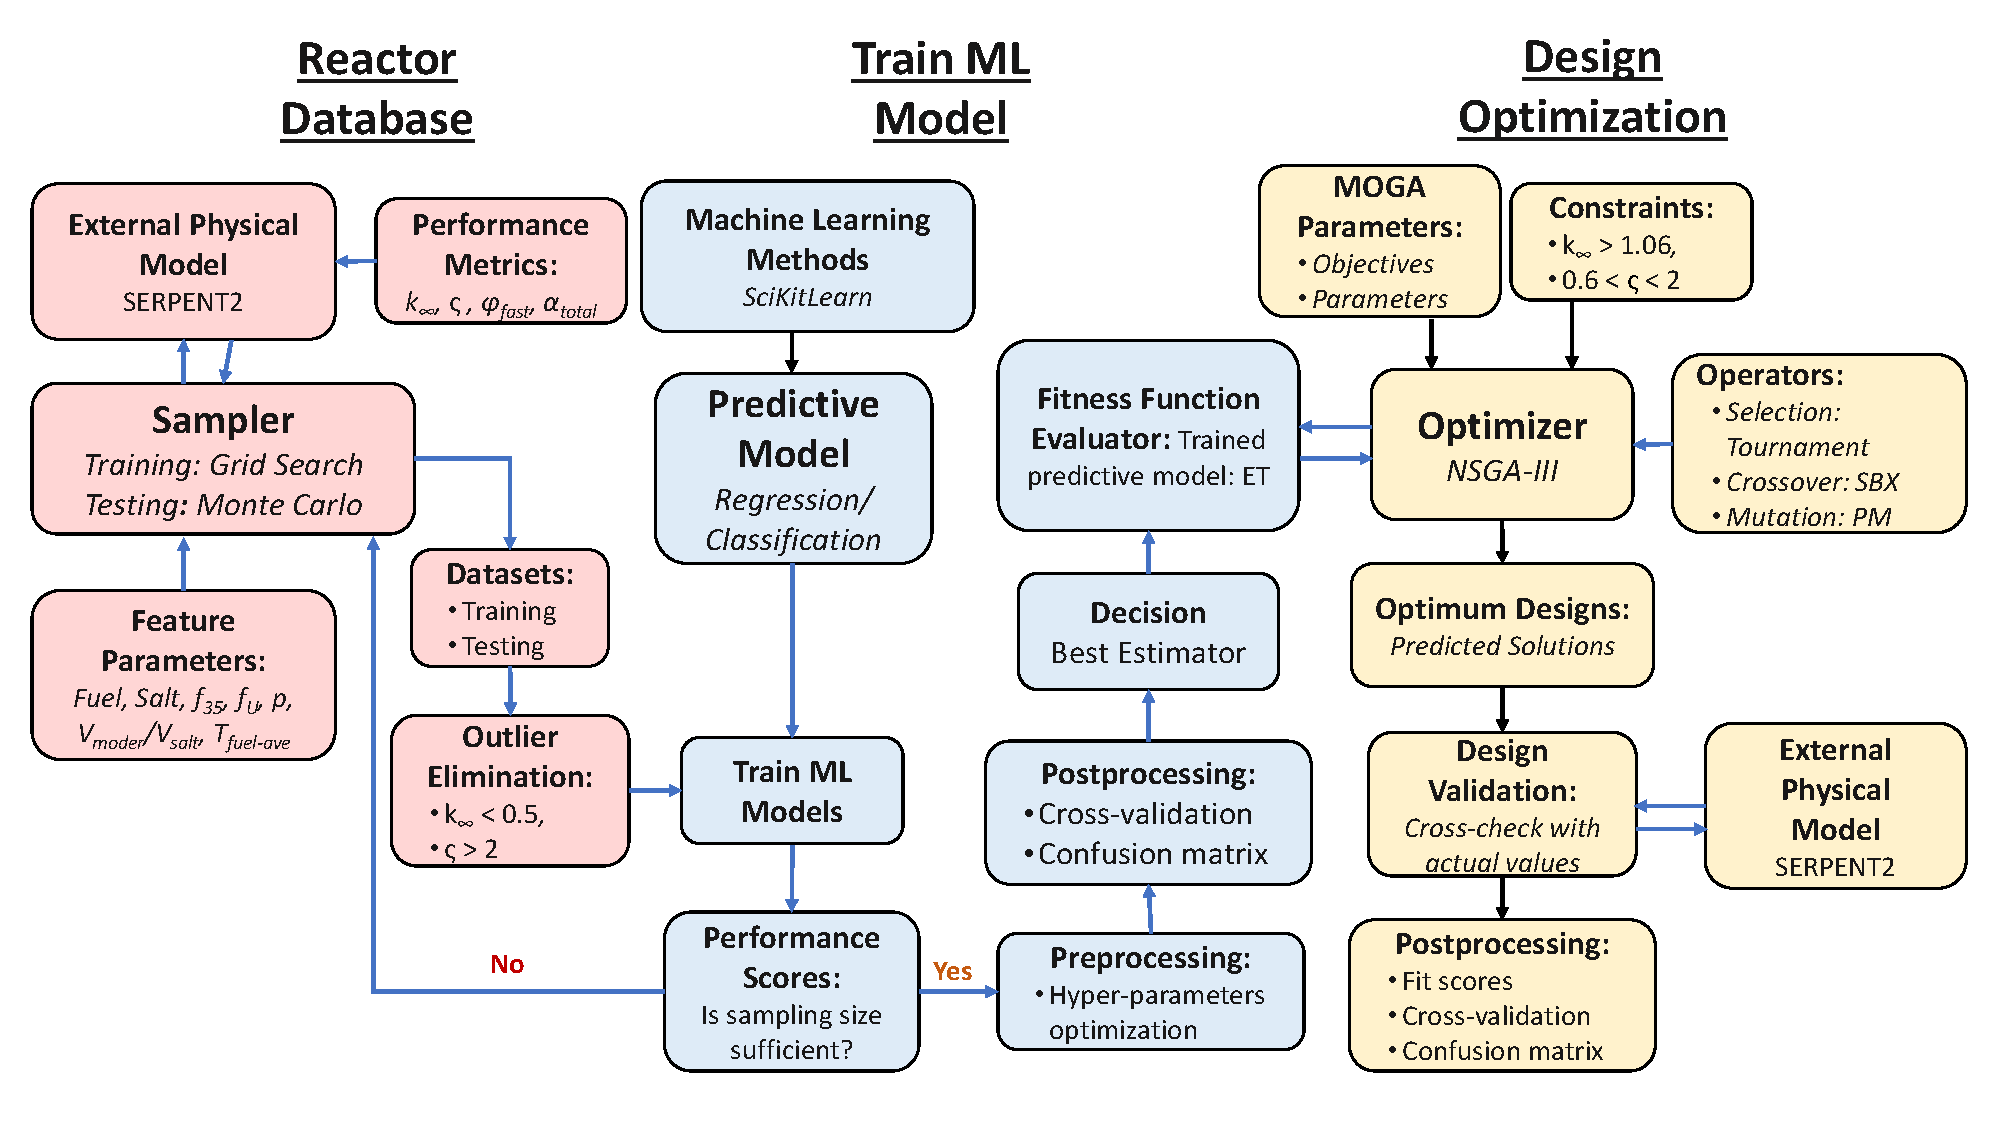
\includegraphics[trim = 0 20 0 20, clip,
	width=\textwidth]{images/computational_flowchart.pdf}
	\caption{Computational flowchart of the Plankton code}
	\label{fig:flowchart}
\end{figure}

 

\subsection{Plankton}

\subsubsection{Database Generation}

The database generation is the step in which samplings in datasets are created
and, training and testing datasets are produced based on two distinctive
sampling strategy, Grid sampling and Monte Carlo.

The grid sampling strategy, the simplest exploration approach to explore an
uncertain domain, was used to obtain the training dataset. It constructs an
N-dimensional grid in which each dimension accounts for a single feature
parameter. A sample in the dataset represents a specific node in the grid.

In contrast to the grid strategy, a test dataset was generated by the Monte
Carlo technique in which the value of each variable is randomly determined
between the lower and upper limits. As the size of samplings has a significant
effect on fitting scores of the training data, the determination criteria for
the size of datasets were explicitly defined in the learning curve section.
Therefore, the estimation of the optimum training sample size is performed by
the 'learning$\_$curve' tool in conjunction with 'ShuffleSplit', which examines
the change in the validation and training score of an estimator for which the
number of training samples varies.

Computational steps performed in database generation phase:
\begin{itemize}
	\item Initialize the feature parameters, properties of which are given in
	Table~\ref{table:features}, for the grid search technique and Monte Carlo
	method.
	\item Prepare the input files for the reactor physics code for neutron
	transport calculation and simulate each sample in training and testing datasets.
	\item Calculate the performance metrics and extract them from the code output.
	\item Supply the prepared reactor database, a set of training/testing samples
	which comprise the feature parameters with corresponding performance metrics, to
	the machine learning phase.
\end{itemize}

\subsubsection{Machine Learning}

In this part, we scoped out various regressors and classifiers from \gls{ML}
methods with the scikit-learn python package \cite{Ped2011}.
Table~\ref{table:AImethods} lists \gls{ML} methods including semi-supervised and
supervised methods such as \gls{NN}, ensemble, linear, \gls{SVM}, decision tree,
naive bayes, and neighbor-based methods. Because there is more than one
performance metric, the estimators need a built-in or external
multi-class/multi-label support. We therefore used the multi-target multi-output
method in regression and multi-label multi-output method in classification when
necessary. In this context, either 'MultiOutput' or 'OneVsRest' tools (e.g., for
\gls{SV} classifier) were utilized. We performed a comprehensive performance
assessment by examining various regression and classification metrics given in
Table~\ref{table:MLmetrics}. Prior to regression/classification analyses, we
standardized our datasets by the MinMaxScaler scaler that scales each feature
parameter between zero and one.

For the optimization of the hyper-parameters of the estimators, we performed an
exhaustive search over specified parameter values using GridSearchCV within the
scikit-learn module to further improve the scores of estimators.

Computational steps performed in machine learning phase:
\begin{itemize}
	\item As a starting point, use diverse \gls{ML} methods, listed in
	Table~\ref{table:AImethods}, from the scikit-learn tool.
	\item With the default settings of hyper-parameters, assess the potential
	estimators to be used in training just by looking into their fit performances
	and exclude the worst ones from the list of the potential estimators.
	\item Analyze the learning curves of the selected estimators to understand
	the optimal sample size required for a high-quality training.
	\item Make a hyper-parameter optimization for the selected estimators to
	further improve the estimators' scores.
	\item Eliminate the outliers for which the performance metrics which seem
	impracticable from the viewpoint of designing a reactor and are out of interest,
	to further improve the estimators' scores, focusing on only the feasible
	solution domain.
	\item Select the best estimator(s) according to their fitting scores.
	\item For better understanding of the selected estimators' capability, get
	the final scores of the estimators, cross-validate the results of the
	regressors, and draw confusion matrices of the classifiers.
	\item Supply the best estimator(s) (along with the optimized
	hyper-parameters) to the design optimization phase to predict the performance
	metrics of the objective functions. 
\end{itemize}

%%%%%%%%%%%%%%%%%%%%%%%%%%%%%%%%%%%%%%%%
\begin{table}[ht!]
	\centering
	\caption{Examined \gls{ML} methods \cite{Ped2011}} 
	\begin{tabular}{ll}
		\hline
		\textbf{Method} & \textbf{Estimator}    \\ \hline
		Ensemble  & \gls{RF}, Bagging (B)  \\
		& AdaBoost (AB), \gls{ET} \\
		& GradientBoosting (GB)   \\
		Linear    & ElasticNet (EN), Perceptron (P), Ridge (R) \\
		& StochasticGradientDescent (SGD)  \\
		& Lasso (L), LassoLars (LL), Logistic (Log) \\
		Naive Bayes     & GaussianNB (GNB), BernoulliNB (BNB)\\
		Neighbor-Based  & \gls{KN} \\
		\gls{SVM} & \gls{SV} \\
		\gls{NN}  & \gls{MLP} \\
		\gls{DT}  & \gls{DT}  \\
		Semi-Supervised & LabelPropagation (LP) \\ \hline
	\end{tabular}
	\label{table:AImethods}
\end{table}
%%%%%%%%%%%%%%%%%%%%%%%%%%%%%%%%%%%%%%%%
\begin{table}[ht!]
	\centering
	\caption{Metrics for performance assessment of estimators \cite{Ped2011}} 
	\resizebox{\textwidth}{!}{%
		\begin{tabular}{ll}
			\hline
			\textbf{Regression}                  & \textbf{Classification}                  \\ \hline
			fit score (fit$\_$score)             & fit score (fit$\_$score)                 \\
			mean square error (MSE)              & average precision (AP)                   \\
			mean absolute error (MAE)            & ranking-based average precision (LRAPS)  \\
			explained variance regression (EVR)  & label ranking loss (LRL)                 \\
			coefficient of determination (R$^2$) & average Hamming loss (HL)                \\
			& computed area under the receiver         \\
			& operating characteristic curve (ROC-AUC) \\ \hline
	\end{tabular}}
	\label{table:MLmetrics}
\end{table}
%%%%%%%%%%%%%%%%%%%%%%%%%%%%%%%%%%%%%%%%

\subsubsection{Design Optimization}

In the final stage of the channel design, we aimed at finding the optimal
designs. We implemented a multi-variable multi-objective evolutionary algorithm.
We selected this method because optimization methods such as gradient-based or
non-linear least-square do not accept discrete and non-numeric variables. We
opted for an optimization method appropriate to the problem's behavior which
manifests a convex structure rather than a linear relationship.

We defined the number of generations as a convergence stopping criterion. After
finding the optimum designs with Plankton's ML methods, we rerun Serpent tool
with the optimal design feature parameters to crosscheck the solutions. Thus, we
performed additional neutron transport calculations for the optimal designs via
the reactor physics code, used to generate the reactor database. Acceptance
criteria for the accuracy of the optimal designs was selected as:
\begin{eqnarray}\label{Eq0}
\dfrac{x_{i,a}-x_{i,p}}{x_{i,a}} \leq 5%
\end{eqnarray}
where $x_{i,a}$ is the actual value of i$th$ metric and $x_{i,p}$ is the predicted 
value of i$th$ metric.

Computational steps performed in design optimization phase:
\begin{itemize}
	\item Initialize the \gls{MOGA} parameters including decision variables,
	operators, number of generations, initial population size, crossover rate
	and mutation ratio.
	\item Define the constraints for the performance metrics which would
	eliminate undesired designs.
	\item Use a \gls{GA} method, which are naturally
	limited by the problem, consistent with the structure of the feature parameters.
	\item Couple the estimator(s) to the \gls{GA} method to calculate the
	performance metrics of the objective functions, without running a reactor physics
	code.
	\item Iterate this \gls{ML}-\gls{GA} coupled system until either the
	constraints are met or the solutions are converged to one of the predefined
	criteria. 
	\item Verify the pareto-front (predicted) solutions by calculating actual
	values.
\end{itemize}

\subsection{Channel Design with Plankton}

\subsubsection{Design Parameters}

We applied the suggested method to a single fuel channel \gls{MSR} geometry with
square unit cell approximation to use in a basic geometry with the least number
of feature parameters and performance metrics. An illustration of the channel
geometry is shown in Figure~\ref{fig:channel}. Feature parameters describing the
material and geometry properties of the single channel were selected as fuel
type, salt type, $^{235}$U fraction ($f_{35}$) in U, U fraction ($f_{U}$) in
heavy metal, channel-to-channel pitch length ($p$), moderator-to-salt volume
ratio ($\xi$), and average fuel-salt temperature ($T_{ave}$) along the channel.
We varied the variables between upper and lower bounds described in
Table~\ref{table:features}. The $^{235}$U fraction in U was limited to 20 wt.\%
which is the maximum limit for \gls{HALEU}. For the fuel types other than U fuel
type, U content in heavy metal varies from 10 to 90 wt.\%. The maximum $p$,
based on \gls{ORNL}'s \gls{MSRE} design, was set to 16 cm. The $\xi$ variable
was calculated from the ratio of pitch to fuel salt radius between 0.274
(p/D$_{fuel}$ = 1) and 10.46 (p/D$_{fuel}$ = 3).

We studied three different fuel types, U, U-Th and U-Pu in this work. Th in U-Th
contains only $^{232}$Th isotope whereas Pu in U-Pu comes from the weapon-grade
Pu constituting the following isotopes: $^{238}$Pu (0.05 at.\%), $^{239}$Pu
(94.3 at.\%), $^{240}$Pu (5 at.\%), $^{241}$Pu (0.6 at.\%) and $^{242}$Pu (0.05
at.\%). It is assumed that there is no $^{234}$U in U as a parasitic absorber.

We examined three types of different salts widely used in prototype reactors by
various companies (Terrestrial Energy, Terrapower, Thorcon, etc.): LiF-BeF$_2$,
NaF-BeF$_2$, and NaCl. The upper value of average fuel-salt temperature
($T_{ave}$) is set to 1200 K while its base temperature used to calculate the
total feedback coefficient of reactivity is 900 K. As the temperature is the
main driver for fuel salt density and Doppler effect on feedback, salt density
variation with the $T_{ave}$ was taken into account based on the reports
\cite{Janz1988, Jerden2019}.

The most critical performance metrics are the infinite multiplication factor
($k_{\infty}$), conversion ratio ($\varsigma$), fast flux ($\phi_{fast}$)
incident on the graphite moderator and total feedback coefficient
(${\alpha_{total}}$). However, ${\alpha_{total}}$ was not considered as
performance metrics in ML phase as it can be calculated promptly and accurately
from Eq. \protect\ref{Eq1} using $k_{\infty}$, thus being calculated at the end
of the design optimization phase.

In classification analysis, a channel design was labeled with different labels
according to its spectrum, type, criticality condition and positive or negative
sign of the feedback coefficient. Accordingly, we addressed any channel design
as breeder type when $\varsigma \geq 1.0$, as fast spectrum when \gls{EALF}
$\geq 1eV$, as supercritical condition when $k_{\infty} \geq 1.0$, and as
positive feedback when ${\alpha_{total}} \geq 0.0$. For the opposite of these
conditions, the design is labeled as burner type, thermal spectrum, sub-critical
condition, and negative feedback, respectively.

Associated with the channel design, we made the following approximations,
simplifications and approaches involved in the model/method development:
\begin{itemize}
	\item The unit cell approximation with a square lattice was chosen to represent
	the single channel geometry. It is an effective geometry structure for
	periodicity.
	\item The fuel-salt is assumed to be stationary, by neglecting
	thermal-hydraulic effects such as delayed neutron precursor movement.
	\item Calculations were performed for initial fuel loading assuming fresh fuel.
	\item Total heat generation	rate along the channel is expressed in terms of an
	arithmetic average of the inlet and outlet temperatures, i.e., $T_{ave}$ =
	($T_{in}$+$T_{out}$)/2, thereby, making the design independent from the length
	of the channel.
\end{itemize}

Using these approximations, we eliminated four interdependent variables: inlet
and outlet temperatures, heat generation rate, and channel length, to the
average temperature definition. We reduced the total number of feature
parameters from eleven to seven parameters.

%%%%%%%%%%%%%%%%%%%%%%%%%%%%%%%%%%%%%%%%
\begin{figure}[ht!]
	\centering
	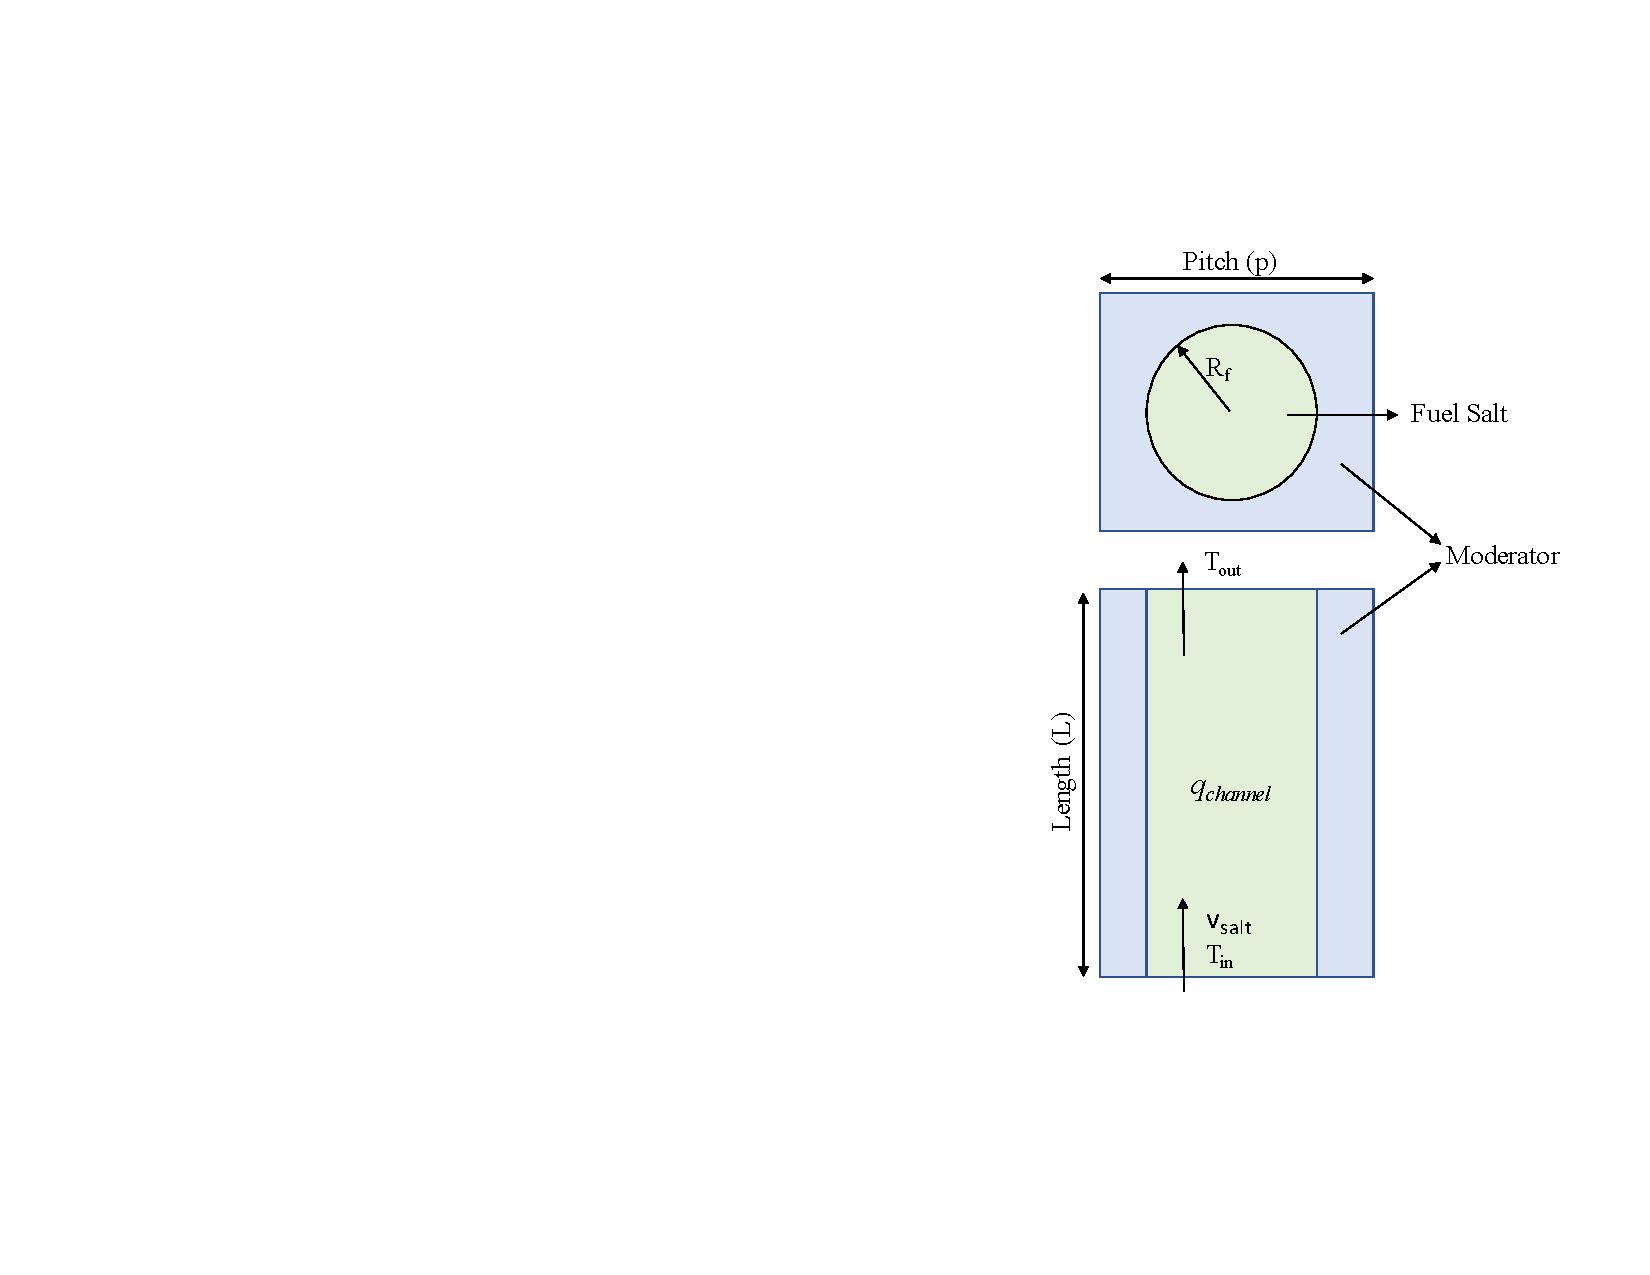
\includegraphics[trim=500 140 0 100, clip,
	scale=0.6]{images/single_channel.pdf}
	\caption{Single fuel channel representation}
	\label{fig:channel}
\end{figure}
%%%%%%%%%%%%%%%%%%%%%%%%%%%%%%%%%%%%%%%%
\begin{table}[ht!]
	\centering
	\caption{Feature parameters for database generation}
	\begin{tabular}{lllll}
		\hline
		\textbf{Variable} & \textbf{Distribution} & \textbf{Material types} &
		& \textbf{Steps} \\ \hline
		Fuel Type & Discrete   & U, U-Th, U-Pu & & 3 \\
		Salt Type & Discrete   & LiF-BeF$_2$, NaCl, & NaF-BeF$_2$  & 3 \\
		&  & \textbf{Lower value} &\textbf{Upper value} &  \\ 
		$f_{35}$  & Continuous  & 1 wt.\%   & 20 wt.\% & 10 \\
		$f_{U}$   & Continuous  & 10 wt.\%  & 90 wt.\% & 9 \\
		$p$       & Continuous  & 1 cm      & 16 cm & 10 \\
		$\xi$     & Continuous  & 0.274 & 10.46 & 10 \\
		$T_{ave}$ & Continuous  & 900 K     & 1200 K & 5 \\ \hline
	\end{tabular}
	\label{table:features}
\end{table}
%%%%%%%%%%%%%%%%%%%%%%%%%%%%%%%%%%%%%%%%

\subsubsection{Optimization Parameters}

We used the \gls{NSGAIII} \cite{deb2014, jain2014} from the pymoo tool
\cite{pymoo2020} as an optimizer with the \gls{SBX} and \gls{PM} operators. The
population size and number of generations were set to 150 and 5000,
respectively. Tournament selection, in which a set of chromosomes are selected
randomly and then the fittest chromosomes are selected for further operation,
was employed to select the fittest candidates from the current generation.

Several independent constraints imposed by the basic requisites of a \gls{MSR}
design were implemented to the solution objectives in accordance with the
references \cite{rykhlevskii2019, betzler2017, ashraf2019} in the following way:
$k_{\infty}$ is greater than 1.06 to make up for neutron leakage; $\varsigma$ is
higher than 0.6; and $\phi_{fast}$ per source neutron on graphite in which the
maximum value is calculated to be about 100 is less than 50.

In the optimization problem, the feature parameters were assigned as decision
variables while the performance metrics were assigned as solution objectives (or
objective functions). The $k_{\infty}$ and $\varsigma$ metrics were maximized
while the $\phi_{fast}$ was minimized.

\subsubsection{Neutronic Simulator}

We employed a Monte Carlo neutron transport tool, Serpent 2 (2.1.30)
\cite{Lep2014} to compute the performance metrics defined in design parameters
section. It uses ENDF/B-VII.0 \cite{chadwick2006} as the neutron cross-section
library along with S(${\alpha}$, ${\beta}$) thermal scattering libraries. In the
simulator, neutron population per cycle, passive cycle, and active cycle were
set to 2000, 50, and 100, respectively, to yield a computational standard error
of less than 100 pcm in the $k_{\infty}$. A two-group neutron energy structure
for the calculation of $\phi_{fast}$ on the moderator was used and lower and
upper energy boundaries for the fast region were set to 0.625 eV and 20 MeV,
respectively. The $k_{\infty}$, $\varsigma$, and $\phi_{fast}$ metrics were
directly extracted from the output file whereas ${\alpha_{total}}$ was
calculated by Eq. \protect\ref{Eq1}:
\begin{eqnarray}\label{Eq1}
\alpha_{total} = \dfrac{\partial\rho}{\partial T} \approx
\dfrac{\Delta\rho}{\Delta T}=\dfrac{\rho-\rho_b}{T-T_b}
\end{eqnarray}
where $\rho$ is the reactivity, $\rho_b$ is the reactivity at the base
temperature, $T$ is the temperature, and $T_b$ is the base temperature. However,
we purposefully avoided using $\partial \rho /\partial T$ in
estimating/predicting the feedback coefficient as ${\alpha_{total}}$ goes to
infinity when $T_{ave}$ is very close to the base temperature, resulting
problematic outputs. Instead, we used $\partial k$(mk) and converted to
${\alpha_{total}}$ at the end of the calculations. For the energy spectrum
classification of the reactor, the \gls{EALF}  value extracted from the output
file was used.

\subsubsection{Datasets}
In this work, a total training sample size of 285000 and a total test sample
size of 8000 were used.


